\section{Graph Construction Implementation}
\label{sec:4_5}

The graph construction pipeline transforms entity relationships into a PyTorch Geometric HeteroData structure, implemented in \texttt{src/features/graph\_builder.py}.

\begin{figure}[htbp]
    \centering
    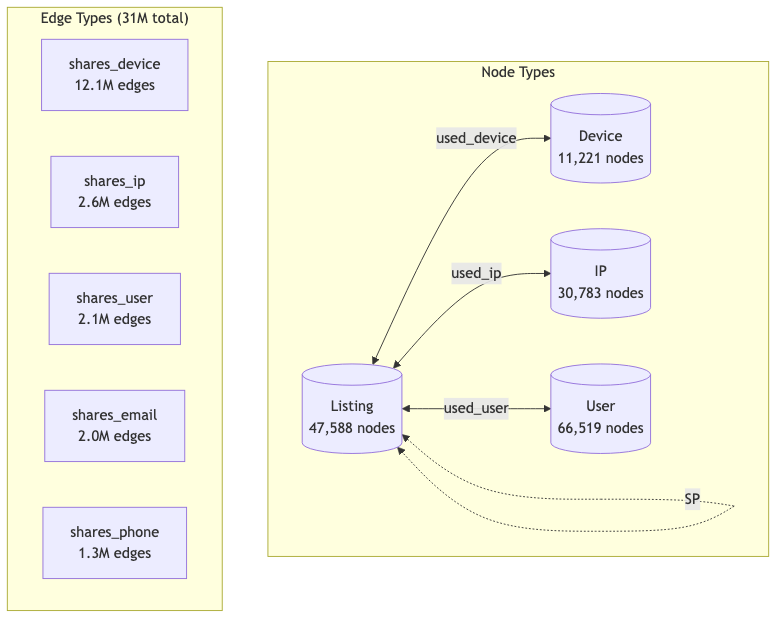
\includegraphics[width=\textwidth]{figures/fig_4_4_4_1.png}
    \caption{Heterogeneous Graph Structure: Node types and edge types}
    \label{fig:4_3}
\end{figure}

\subsection{GraphBuilder Class}
\label{sec:4_5_1}

The \texttt{HeterogeneousGraphBuilder} constructs graphs with multiple node types (Listing, User, Device, IP) and edge types encoding entity-sharing relationships, following the heterogeneous graph framework \cite{hu2020heterogeneous}. While recent advances \cite{yang2024heterogeneous} explore sophisticated heterogeneous architectures with adaptive relation weighting, our implementation employs PyTorch Geometric's standard message-passing approach for computational efficiency at scale. Algorithm~\ref{alg:graph_construction} describes the construction process:

\begin{algorithm}[H]
\caption{Heterogeneous Graph Construction}
\label{alg:graph_construction}
\begin{algorithmic}[1]
\REQUIRE Event dataframe $\mathcal{D}$, temporal cutoff date $t_{cutoff}$
\ENSURE Heterogeneous graph $\mathcal{G}$ with node features and entity-sharing edges
\STATE Filter events: $\mathcal{D}' \gets \{\mathbf{e} \in \mathcal{D} : \mathbf{e}.timestamp \leq t_{cutoff}\}$
\STATE Initialize heterogeneous graph structure $\mathcal{G} \gets \emptyset$
\STATE Extract 44-dimensional node features for each listing from $\mathcal{D}'$
\STATE $\mathcal{G}.nodes[``listing''].features \gets \text{NodeFeatures}(\mathcal{D}')$
\FOR{each $entity\_type \in \{device, IP, email, phone, user\}$}
    \STATE Build sharing edges: $\mathcal{E}_{entity} \gets \text{ConnectSharing}(\mathcal{D}', entity\_type)$
    \STATE Add edge type to graph: $\mathcal{G}.edges[(``listing'', ``shares\_entity'', ``listing'')] \gets \mathcal{E}_{entity}$
\ENDFOR
\RETURN $\mathcal{G}$ with $\sim$31M edges across 5 edge types
\end{algorithmic}
\end{algorithm}

\textbf{Temporal Filtering:} Edges are created only from events before the cutoff date, ensuring the training graph reflects information available at training time. The inference graph extends the cutoff to include test period events. Complete implementation details are provided in Appendix~B.

\subsection{Node Feature Preparation}
\label{sec:4_5_2}

Node features combine 36 base features with 8 temporal encoding features (days\_since\_start, relative\_position, hour\_sin/cos, weekday\_sin/cos, recency) for a total of 44 dimensions per listing node.

\textbf{Neighbor Sampling:} The dense graph (31M edges) requires sampling during training to manage computational complexity. We employ PyTorch Geometric's \texttt{NeighborLoader} with 2-hop sampling: 15 neighbors at layer 1, 10 neighbors at layer 2, with batch size 512. This approach enables efficient training on the full graph while maintaining local neighborhood structure. Sampling parameters were empirically validated to balance representation quality against training time (see Appendix~B for implementation).
